\section{Methods} \label{sec:methods}

In this section, we detail methodology for benchmark and validation experiments used to empirically assess performance of the prroposed shortcut-enabled reconstruction algorithm.

\subsection{Generation of Benchmark Data}

For our benchmark experiments, we needed a sample large-scale genomes to draw from to perform reconstructions on.
For this purpose, we performed simulations using the Cerebras Wafer-Scale Engine, a recently-introduced 850,000 core hardware accelerator device \citep{TODO}.
Processor elements (PEs) in this architecture are arranged in a grid lattice where each processor is able to execute independently and communicate with neighboring PEs through message-passing, with tight per-core limitations on available memory.

To conduct these simulations, we used an extension of the island-model genetic algorithm framework presented in \citep{moreno2024trackable}.
This framework organizes simulated organisms into independent subpopulations hosted on each PE.
Synchronous tournament selection of size 2 is applied within each PE, and between generations agents are migrated between PEs asynchronously.

%The purpose of this simulation was to generate large-scale data using a simple model that can be explicitly manipulated to explore evolutionary regimes differing substantially in the depth of shared ancestry between organisms (known as phylogenetic richness).

A simple genome model was used, wherein agents were comprised of a single floating point value representing fitness.
Reproduction occured asexually, with this value subject to mutation with TODO probability.
In tournament competitions to select parents for the subsequent generation, the parent was selected according to the higher fitness value with 10\% probability and was otherwise selected randomly.

To generate data representative of different evolutionary conditions, two treatments were applied:
\textbf{adaptive regime} and \textbf{purifying regime}.
Under the adaptive regime, mutations increasing fitness were allowed, introducing the possibility of selective sweeps.
By contrast, the purifying regime treatment allowed only the possibility of deleterious mutations
Previous work with this system demonstrated the purifying regime to exhibit substantially greater phylogenetic richness --- in line with expectation.

Fossil data were sampled on a rolling basis using asynchronous memcpy operations, where a representative agent was copied from device-to-host from each processor element on a rolling basis.
The simulation was run for TODO processor element generation cycles, which took TODO minutes.
A population size of TODO was used, and synchronous generations were used so that over the course of this simulation, TODO replication cycles were used.
Over the course of the simulation, TODO memcopy cycles elapsed.
Real time runtime for each was X and Y.
For full details on the Wafer-Scale Engine, see \citep{moreno2024trackable}.

We used hstrat annotations comprising 64 single-bit markers, managed at runtime using a \texttt{tilted} curation policy, which favors dense retention of more recent marker data.

\subsection{Microbenchmark Experiments}

From this simulation (in both purifying and adaptive versions), we took a random sample of 10 million tips that could be used on a personal computer for various benchmarks, which were inteded to test reconstruction performance.
First, we wanted to determine the asymptotic complexity of our new algorithm; to do this, we ran sub-samples of various sizes through the reconstruction pipeline and measured the time it took in the reconstruction step.
This was done for both adaptive and purifying simulations in order to test different arrangements of data.

We then wanted to compare the performance of this algorithm with the previous naive trie algorithm. We did this by again taking subsamples of the 10 million tips, and running both algorithms on the subsample and timing how long it took to process all the tips. Given that the naive algorithm is significantly slower, our subsample sizes were limited to up to 10,000 tips. 

Because of this, we also wanted to determine the performance of the search table algorithm on larger data, and more importantly, determine the asymptotic complexity of the approach. 
To do this, we took a range of sub-samples from the original sample up to 10 million tips, ran the end-to-end pipeline, and measured the time taken on the reconstruction step alone.
We also performed this process on both adaptive and purifying regimes, so that we could determine if there were potential differences depending on the evolutionary scheme.

These examples were all run on a 2019 MacBook Pro (2.3GHz 8-Core Intel i9, 16GB RAM) using a benchmark script attached with our supplemental material \citep{supplemental}.

\subsection{Macrobenchmark Experiments}

To assess the performance of our approach on large-scale workloads under real-world conditions, we supplemented microbenchmarks focusing on core trie extension and consolidation operations with two macrobenchmark trials comprising the full end-to-end reconstruction pipeline described in Section \ref{sec:pipeline}.
These end-to-end experiments used the \texttt{hstrat.dataframe.surface\_build\_tree} CLI module incorporated in the \texttt{hstrat} library.

These experiments were conducted using the full billion element corpus of sampled genomes from Wafer-Scale Engine simulations.
We performed two trial reconstructions: one using genome data from the adaptive regime treatment and another under the purifying regime treatment.

Reconstructions were conducted on dedicated cluster nodes.
End-to-end experiments used the \texttt{hstrat.dataframe.surface\_build\_tree} CLI module incorporated in the \texttt{hstrat} library.

TODO hardware specs.

\subsection{Validation Tests}

One part of our algorithm we aim to show is that it is essentially equivalent to the naive trie algorithm already implemented.
We have already proven that any decisions it makes could be made by the naive trie algorithm (i.e. it is a valid arbitrary choice made by the algorithm); however, we do not know if they give similar results in practice.

On the other hand, to demonstrate reconstruction accuracy, we used small evolutionary simulations run locally. 
These simulations were relatively simple, running 500 generations where parents replicated and died out, and 500 generations where parents replicated and stayed in the population. These simulations were ran using perfect tracking as implemented in \texttt{phylotrackpy} \citep{dolson2024phylotrack} so that reconstructed phylogenies could be compared with the ground truth.
We then obtained a numerical error measurement using a triplet distance calculation between the ground truth and reconstructed phylogenies \citep{critchlow1996triples}.

\subsection{Algorithm Implementations}

This shortcut-based algorithm is implemented in the \texttt{hstrat} Python package \citep{moreno2022hstrat} as \texttt{hstrat.build\_tree\_searchtable}.
The reconstruction backend is selectable between independent implementations written in either pure Python or in C++, bound via Pybind11 \citep{pybind11}.
Benchmarks comparing the shortcut-enabled approaches to the existing naive approach, implemented in pure Python, used the pure Python backend for the shortcut-enabled approach, to ensure apples-to-apples comparability.
Other benchmarking and validation experiments used the C++ backend, which is expected to be better reflective of how the library will be used in practice, given the inherent speedup and memory savings associated with compiled code.

As suggested by the function name, both shortcut-enabled backends represent trie data using an edge-list table, rather than a node-and-pointer approach, as is the case with the existing naive implementation.
From an algorithmic perspective, tabular and node-and-pointer data structures provide identical properties for traversal and lookup operations.
However, in practice, the former approach is often faster due to fewer memory allocation operations and better cache locality.

At the implementation level, we represent trie shortcuts via additional columns in our edge table.
When a new node is appended, its shortcut edge is initialized identically to its trie edge.
From this point onwards, shortcut edges are used only for traversing the trie, while underlying trie edges -- treated as immutable from node initialization onwards -- are used when reading out the final reconstruction result.

\subsection{Build-time Garbage Collection}

To reduce memory usage for very large phylogeny reconstructions, we supplement the core trie extension and consolidation procedure detailed in Section \ref{sec:algorithm} with an intermittent garbage collection step.
Because genomes are inserted in ascending order of generational depth, trie nodes at a generation with a single child node.
Given that all trie nodes only have a single parent node, such a ``dropped unifurcation node'' can be excised and safely replaced with an edge directly connecting its parent and child.

As currently implemented, we use the presence of modifications to shortcut edges to identify nodes for which corresponding hstrat markers have been dropped.
We note that this does not detect all dropped unifurcations, and an alternate more aggressive approach could be implemented readily by incorporating information as to which markers have been dropped from the marker retention algorithm used at runtime.

At implementation-level, the frequency of ``dropped unifurcation'' garbage collection is provided as a configurable function parameter, and so can be tuned as appropriate for a given use case scenario.
Garbage collection was not necessary for the up to 10 million tip reconstructions evaluated in our microbenchmarking experiment, and so was not performed.
For our macrobenchmark experiments, we ran this procedure at three evenly-spaced intervals during the build process.
Figure \ref{fig:billion-tip-time} details the share of net execution time consumed by purging dropped unifurcations in these trials.

\subsection{End-to-end Phylogeny Reconstruction Pipeline}
\label{sec:pipeline}

\begin{figure*}
% graphic source https://docs.google.com/presentation/d/1CKU1Rtz8Vbk-Std3zFmzBcACf7EBj3amTTOAGKdBluQ
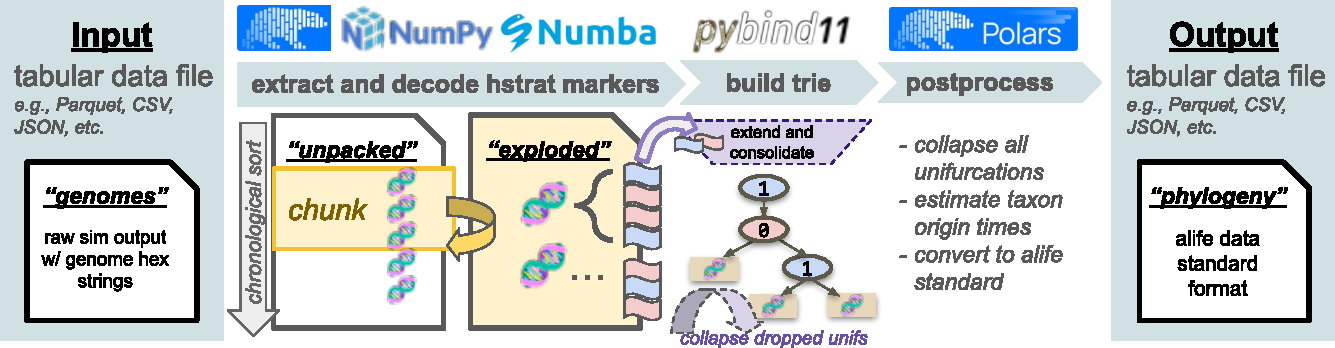
\includegraphics[width=\linewidth]{img/hstratpipeline.pdf}
\caption{\textbf{Schematic of hstrat phylogeny reconstruction pipeline.} TODO.}
\label{fig:hstratpipeline}
\end{figure*}


Figure \ref{fig:hstratpipeline} overviews the full end-to-end pipeline used to construct a phylogeny from raw hstrat-annotated genome data.
First, hstrat annotation data is extracted and decoded.
To take advantage of SIMD parallelism, the decoding of origin times for genome markers is performed using bulk operations orchestrated via NumPy, batched over available processors using the Numba library threading engine.
Due to memory-intensity of the exploded representation, where each genome marker constitutes an individual dataframe row, a chunk size may be configured to limit the amount of data exploded at any one time.
A chunk size of TODO was used for macrobenchmark trials.

Subsequently, decoded marker data is fed batchwise into the trie-building backend.
To ensure full hardware utilization, execution of the core trie-building procedure -- which is single-threaded -- is overlapped with decode/explode work on the upcoming chunk through multiprocessing.
Finally, a phylogeny is extracted from the final trie, converted to alife standard format, and saved to disk.
The Polars library is used for load/save and other pre-/post-processing operations, allowing some operations to be distributed over available processor cores by the underlying threading engine.

\subsection{Software and Data Availability} \label{sec:materials}


Supporting software and executable notebooks for this work are available via Zenodo at TODO \citep{moreno2024hsurf}.
DStream algorithm implementations are also published on PyPI in the \texttt{downstream} Python package, where we plan to conduct longer-term, end-user-facing development and maintenance \citep{moreno2024downstream}.
All accompanying materials are provided open-source under the MIT License.

This project benefited significantly from open-source scientific software \citep{2020SciPy-NMeth,harris2020array,reback2020pandas,mckinney-proc-scipy-2010,waskom2021seaborn,hunter2007matplotlib,moreno2023teeplot}.
